\documentclass[main.tex]{subfiles}
\begin{document}
\section{Analysis of Results}

\subsection{Learned Causal Structure}
% \textcolor{teal}{[Include your graph as a figure.]}
% \begin{table}
\caption{Summary of optimal parameters search for FCI algorithm with corresponding time required for execution. The experiments are ran on 27 variables, sample size 6660 records from UA.}
\label{tab:fci_parameters_time_UA_27_talkmother}
\begin{tabular}{lrrl}
\toprule
CI test & alpha & time & result \\
\midrule
gsq & 0.001 & 17.950 & \ref{fig:fci_gsq_0.001all_UA_27_talkmother} \\
gsq & 0.010 & 23.077 & \ref{fig:fci_gsq_0.01all_UA_27_talkmother} \\
gsq & 0.050 & 446.156 & \ref{fig:fci_gsq_0.05all_UA_27_talkmother} \\
\bottomrule
\end{tabular}
\end{table}

% \begin{table}
\caption{Summary of optimal parameters search for FCI algorithm with corresponding time required for execution. The experiments are ran on 78 variables, sample size 6660 records from UA.}
\label{tab:fci_parameters_time_UA_78_famdec}
\begin{tabular}{lrrl}
\toprule
CI test & alpha & time & result \\
\midrule
gsq & 0.001 & 262.675 & \ref{fig:fci_gsq_0.001all_UA_78_famdec} \\
gsq & 0.010 & 5850.981 & \ref{fig:fci_gsq_0.01all_UA_78_famdec} \\
gsq & 0.050 & 19390.311 & \ref{fig:fci_gsq_0.05all_UA_78_famdec} \\
\bottomrule
\end{tabular}
\end{table}

Figures~\ref{fig:fci_gsq_0.001all_UA_27_talkmother} to~\ref{fig:fci_gsq_0.05all_UA_78_famdec} illustrate the Partial Ancestral Graphs (PAGs) produced by the FCI algorithm under different configurations. For the subset of 27 variables, lower significance levels ($\alpha=0.001$) resulted in relatively sparse graphs, whereas higher values ($\alpha=0.05$) produced denser structures. Across all experiments, key variables like \texttt{talkmother}, \texttt{friendtalk}, and \texttt{lifesat} emerged as central nodes.

\begin{landscape}
\begin{figure}[ht]
    \centering
    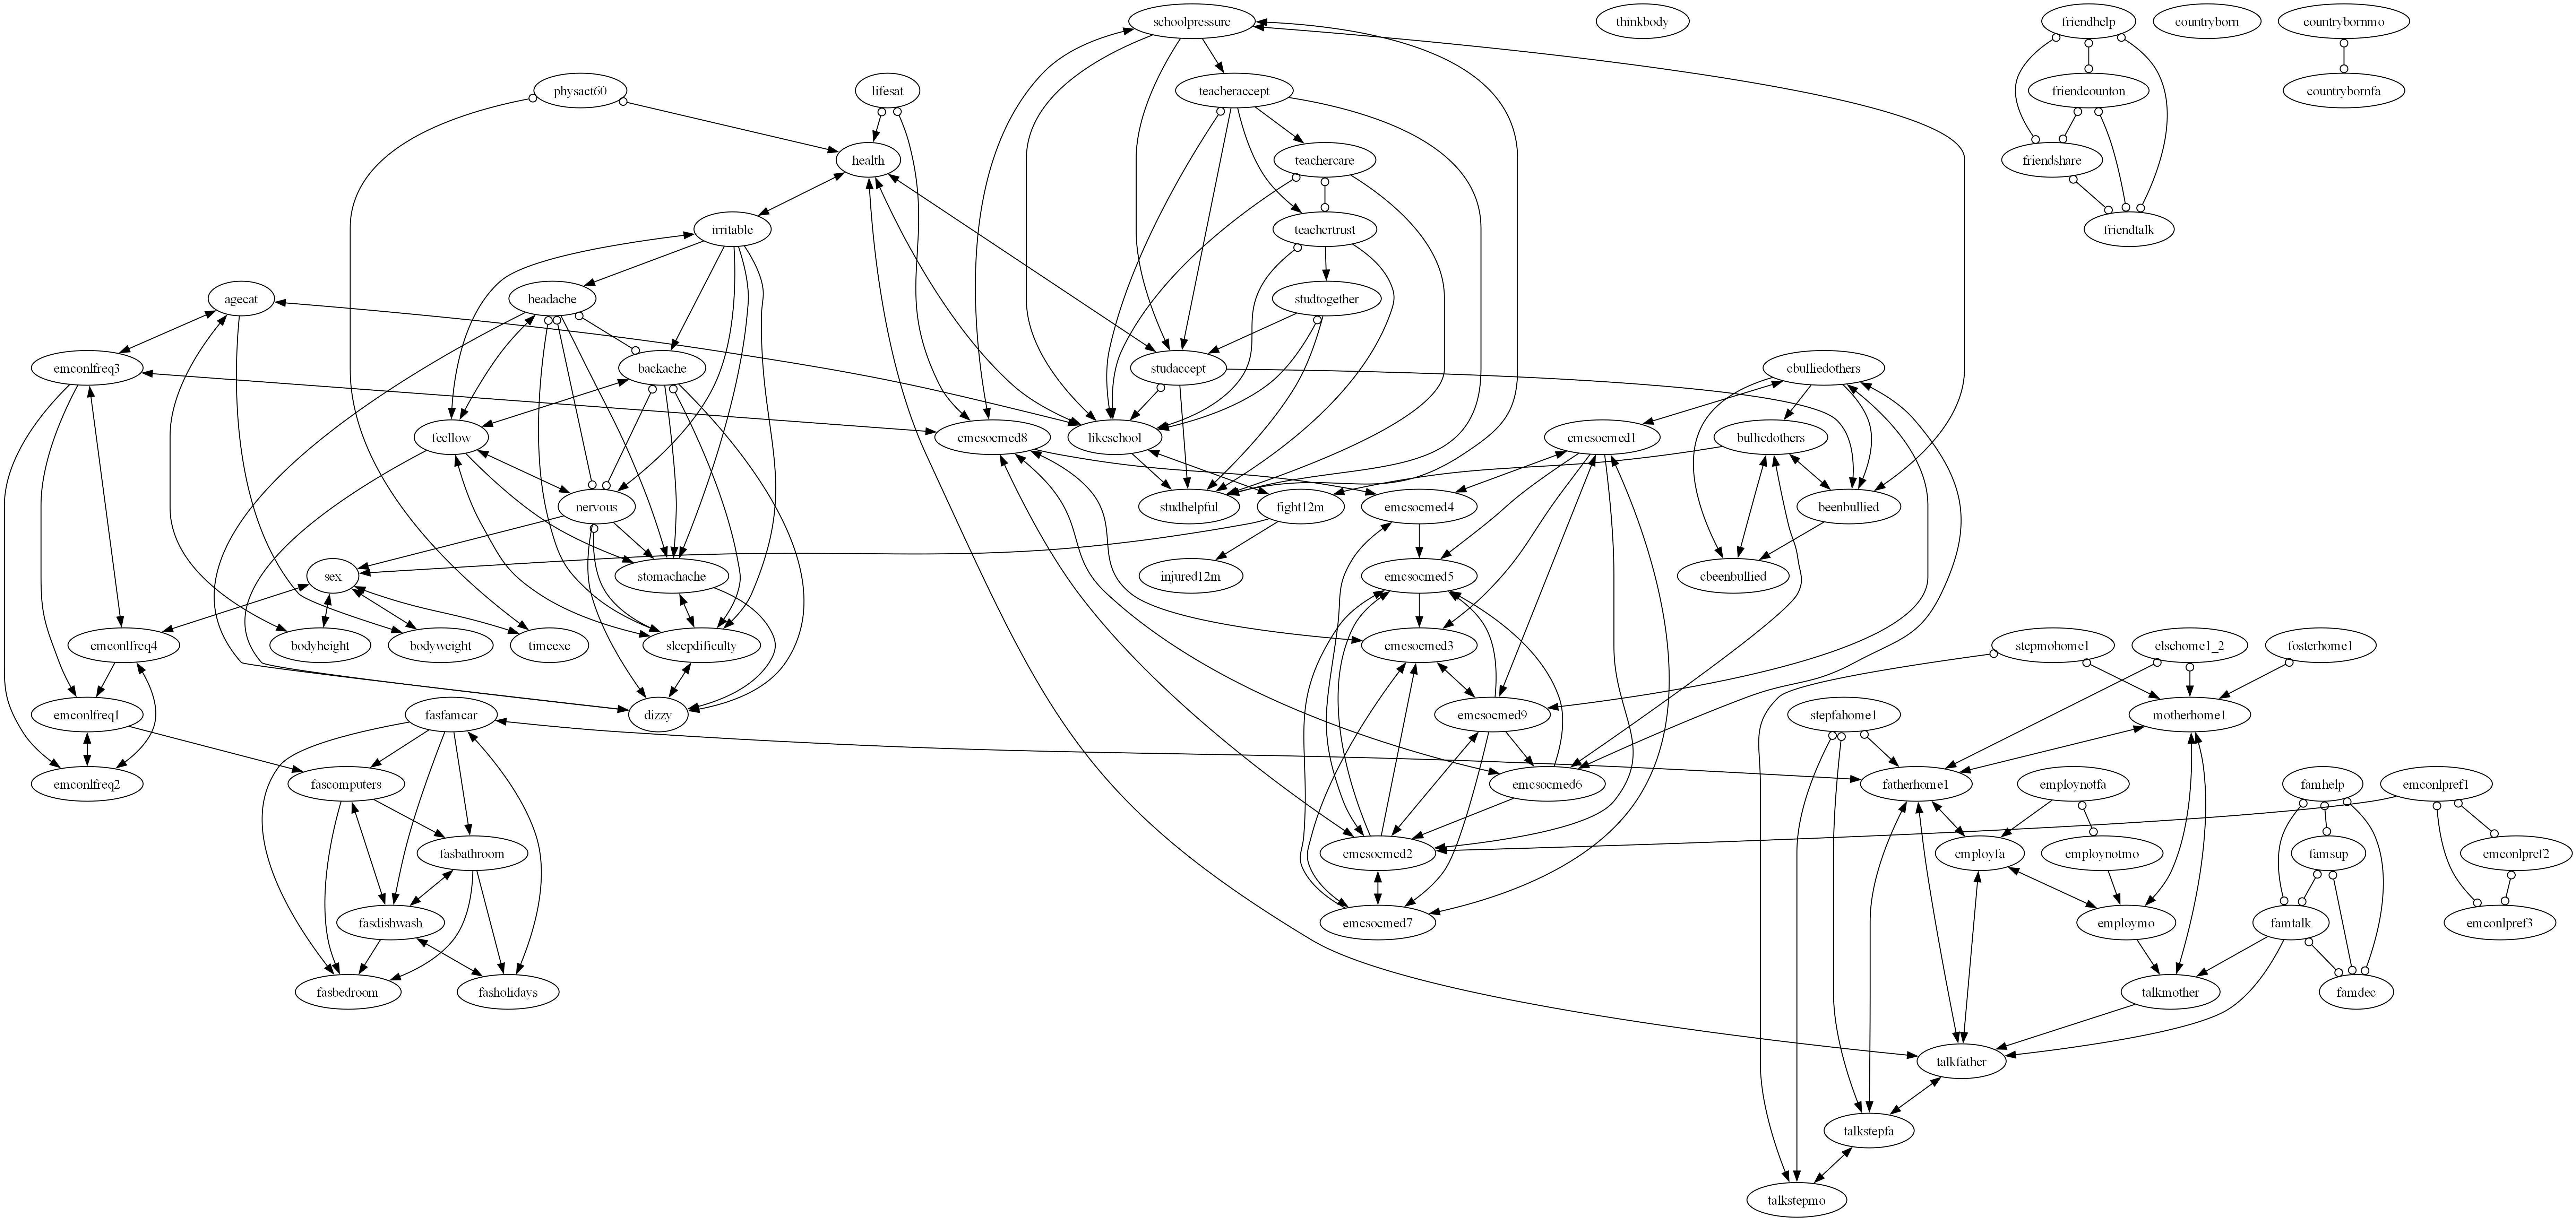
\includegraphics[scale=0.1]{Report/final_report/pictures/FCI_gsq_0.05_all_UA_78_famdec.png}
    \caption{Findings from the FCI algorithm with $G^2$, performed at a significance level of 0.05.}
    \label{fig:fci_gsq_0.05all_UA_78_famdec}
\end{figure}

\end{landscape}


% \begin{figure}[h]
% \centering
% \includegraphics[width=0.8\textwidth]{fci_result.png}
% \caption{Learned PAG using FCI algorithm on HBSC 2018 subset.}
% \end{figure}

\subsection{Interpretation}
Several notable causal relationships can be interpreted from the resulting PAGs:
\begin{itemize}
    \item \texttt{talkmother} $\rightarrow$ \texttt{friendtalk} $\rightarrow$ \texttt{lifesat}: Suggests a pathway from parental communication to peer support, ultimately influencing life satisfaction.
    \item \texttt{schoolpressure} $\rightarrow$ \texttt{beenbullied}: Indicates that higher perceived academic stress may increase susceptibility to bullying.
    \item \texttt{teacheraccept} $\leftrightarrow$ \texttt{likeschool}: Suggests a latent confounder (e.g., school climate or cultural norms) influencing both teacher and school perception.
    \item Bidirected edges such as \texttt{friendshare} $\leftrightarrow$ \texttt{friendtalk} indicate possible shared latent traits such as sociability or emotional openness.
\end{itemize}
\textcolor{teal}{[Explain notable relationships (e.g., parental communication $\rightarrow$ peer trust $\rightarrow$ life satisfaction). Which arrows suggest direct influence? Where are bidirected edges?]}

\subsection{Sensitivity to Parameters}

\begin{table}[hbt]
\centering
\begin{tabular}{lrrrl}
\toprule
Variables & CI test & $\alpha$ & Time (s) & Resulting graph \\
\midrule
27 & $G^2$ & 0.001 & 18 & \ref{fig:fci_gsq_0.001all_UA_27_talkmother} \\
27 & $\chi^2$ & 0.001 & 4516 & \ref{fig:fci_chisq_0.001all_UA_27_talkmother} \\
27 & $G^2$ & 0.010 & 23 & \ref{fig:fci_gsq_0.01all_UA_27_talkmother} \\
27 & $G^2$ & 0.050 & 446 & \ref{fig:fci_gsq_0.05all_UA_27_talkmother} \\
78 & $G^2$ & 0.001 & 263 & \ref{fig:fci_gsq_0.001all_UA_78_famdec} \\
78 & $G^2$ & 0.010 & 5851 & \ref{fig:fci_gsq_0.01all_UA_78_famdec} \\
78 & $G^2$ & 0.050 & 19390 & \ref{fig:fci_gsq_0.05all_UA_78_famdec} \\
\bottomrule
\end{tabular}
\caption{Summary of optimal parameters search for FCI algorithm with corresponding time required for execution. The experiments were run on 6660 records from Ukraine, with different subsets of variables.}
\label{tab:fci_parameters_time_combined}
\end{table}

\begin{figure}[htbp]
    \centering
    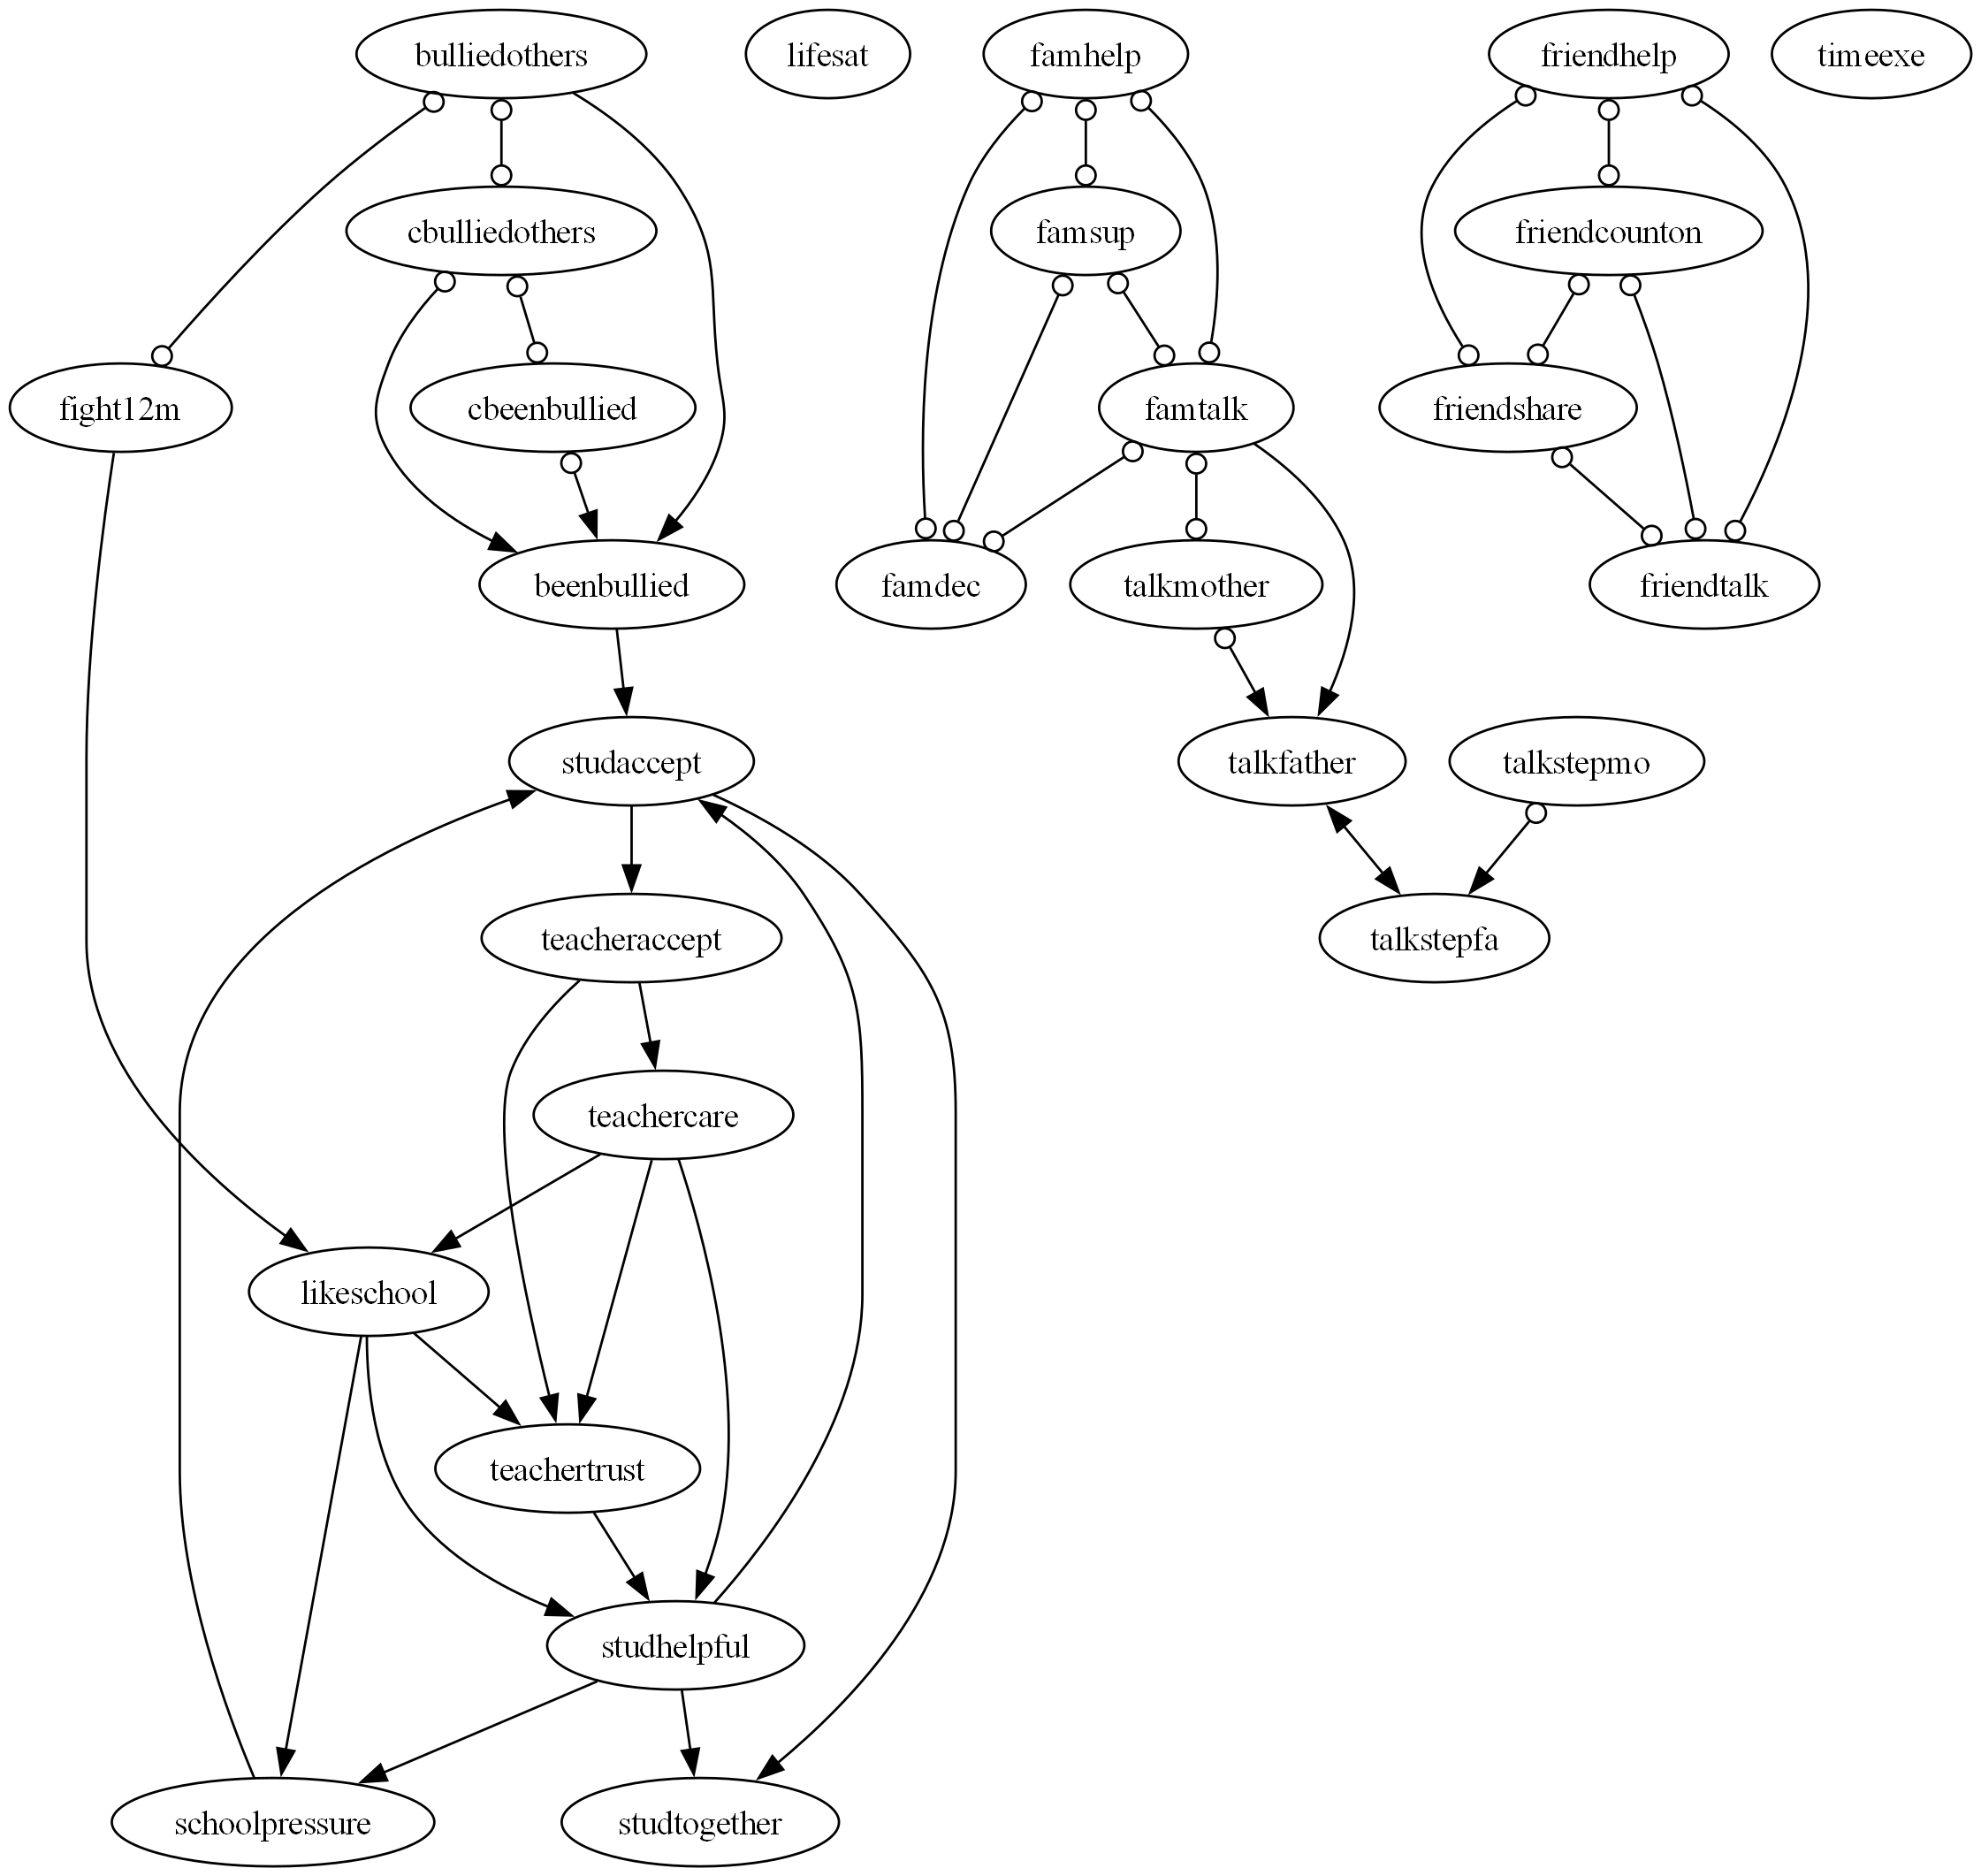
\includegraphics[width=0.8\textwidth]{Report/final_report/pictures/FCI_gsq_0.001_all_UA_27_talkmother.png}
    \caption{Findings from the FCI algorithm with gsq, performed at a significance level of 0.001 for all_UA_27_talkmother.}
    \label{fig:fci_gsq_0.001all_UA_27_talkmother}
\end{figure}

\begin{figure}[htbp]
    \centering
    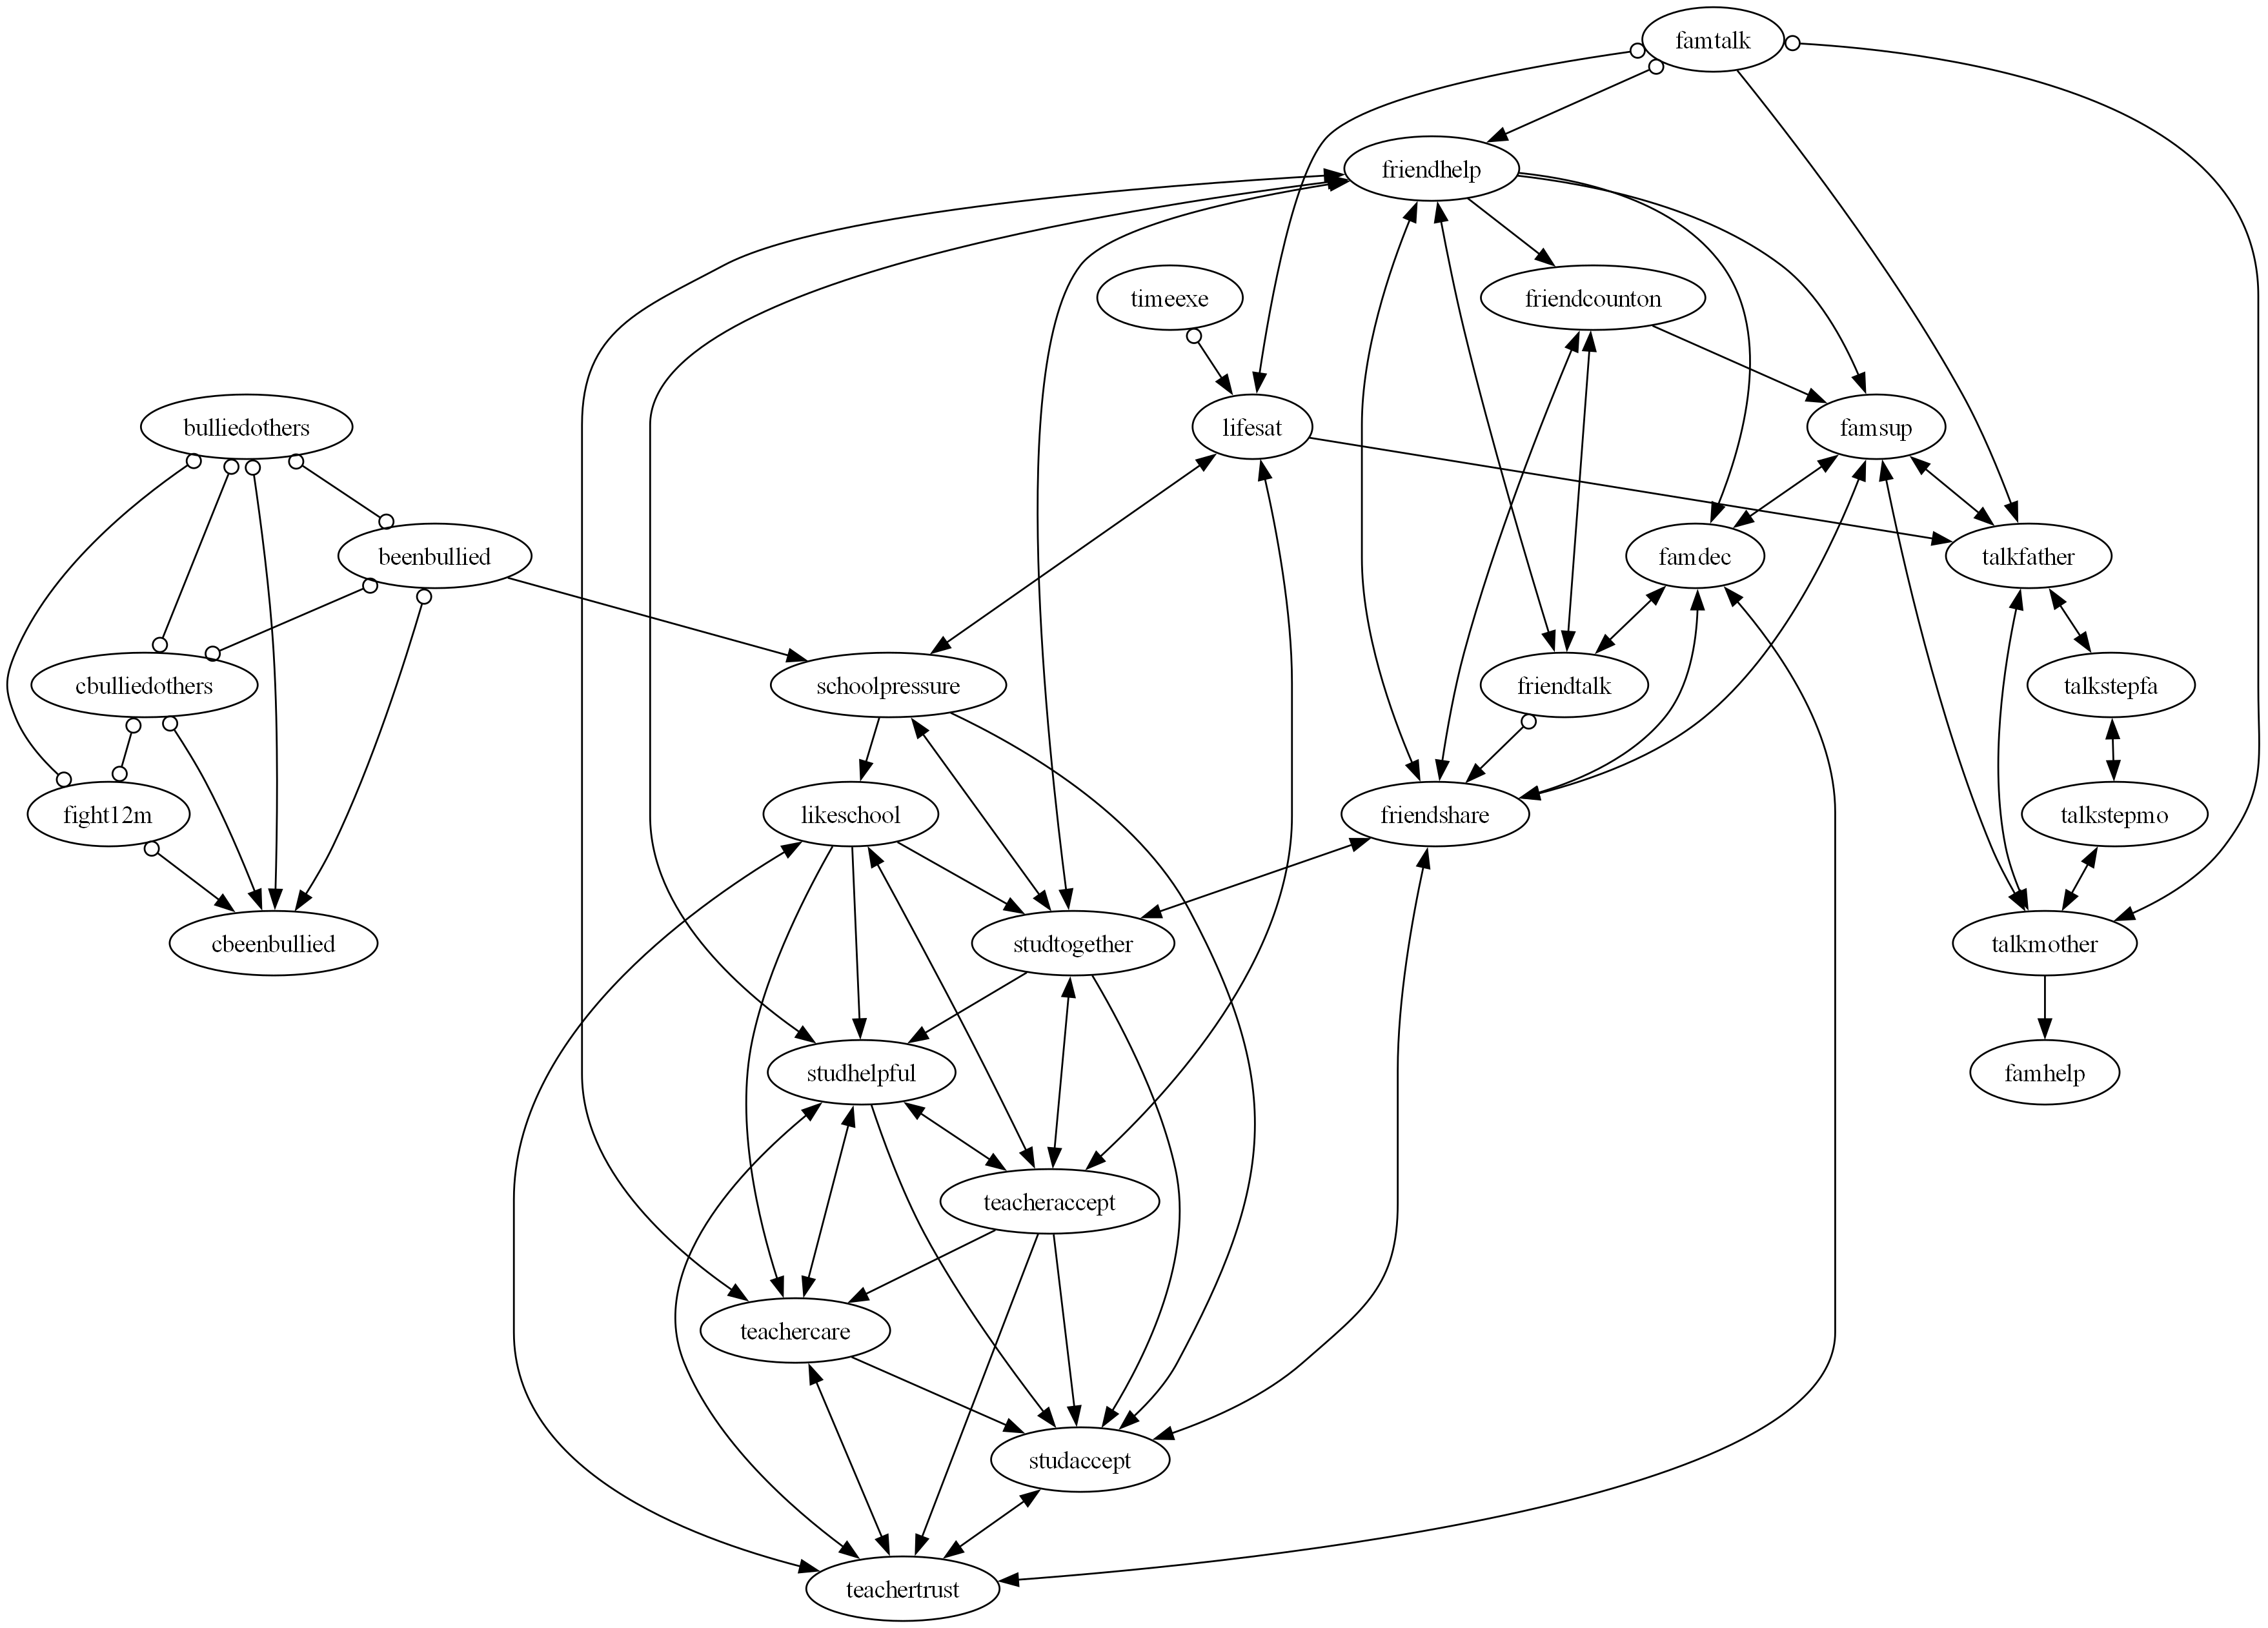
\includegraphics[width=0.8\textwidth]{Report/final_report/pictures/FCI_chisq_0.001_all_UA_27_talkmother.png}
    \caption{Findings from the FCI algorithm with $\chi^2$, performed at a significance level of 0.001.}
    \label{fig:fci_chisq_0.001all_UA_27_talkmother}
\end{figure}

\begin{figure}[htbp]
    \centering
    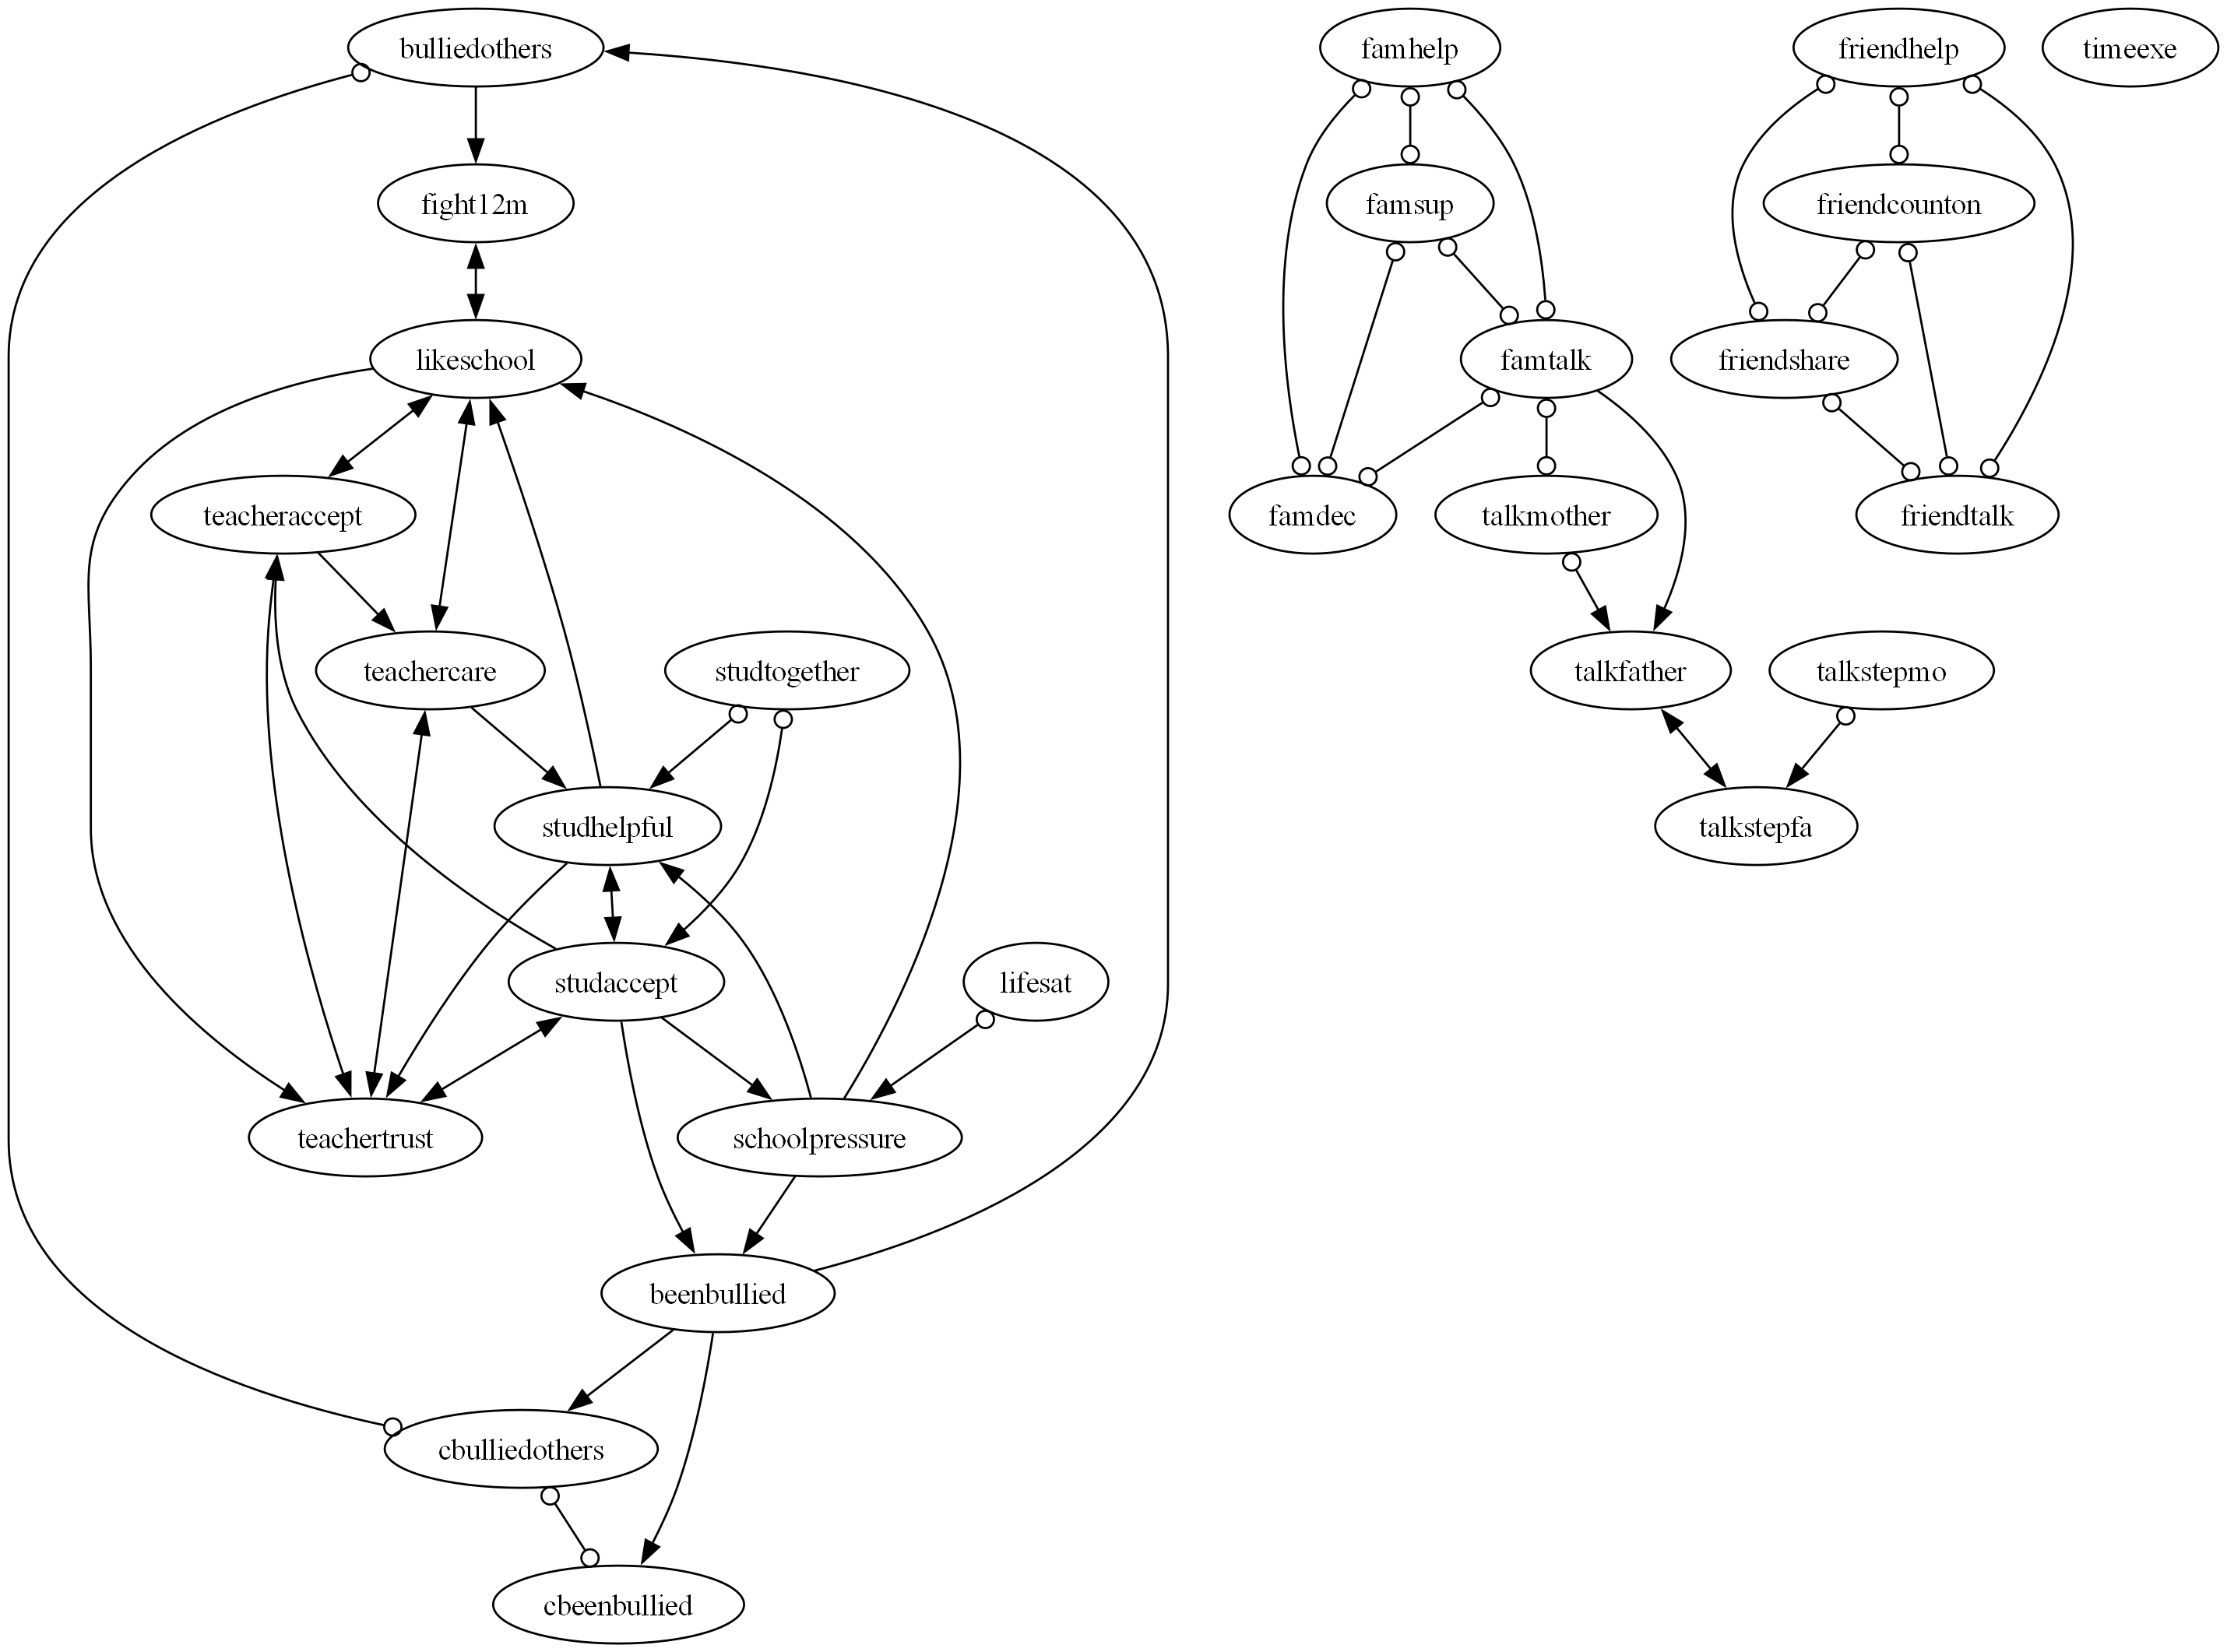
\includegraphics[width=0.8\textwidth]{Report/final_report/pictures/FCI_gsq_0.01_all_UA_27_talkmother.png}
    \caption{Findings from the FCI algorithm with gsq, performed at a significance level of 0.01 for all_UA_27_talkmother.}
    \label{fig:fci_gsq_0.01all_UA_27_talkmother}
\end{figure}

\begin{figure}[htbp]
    \centering
    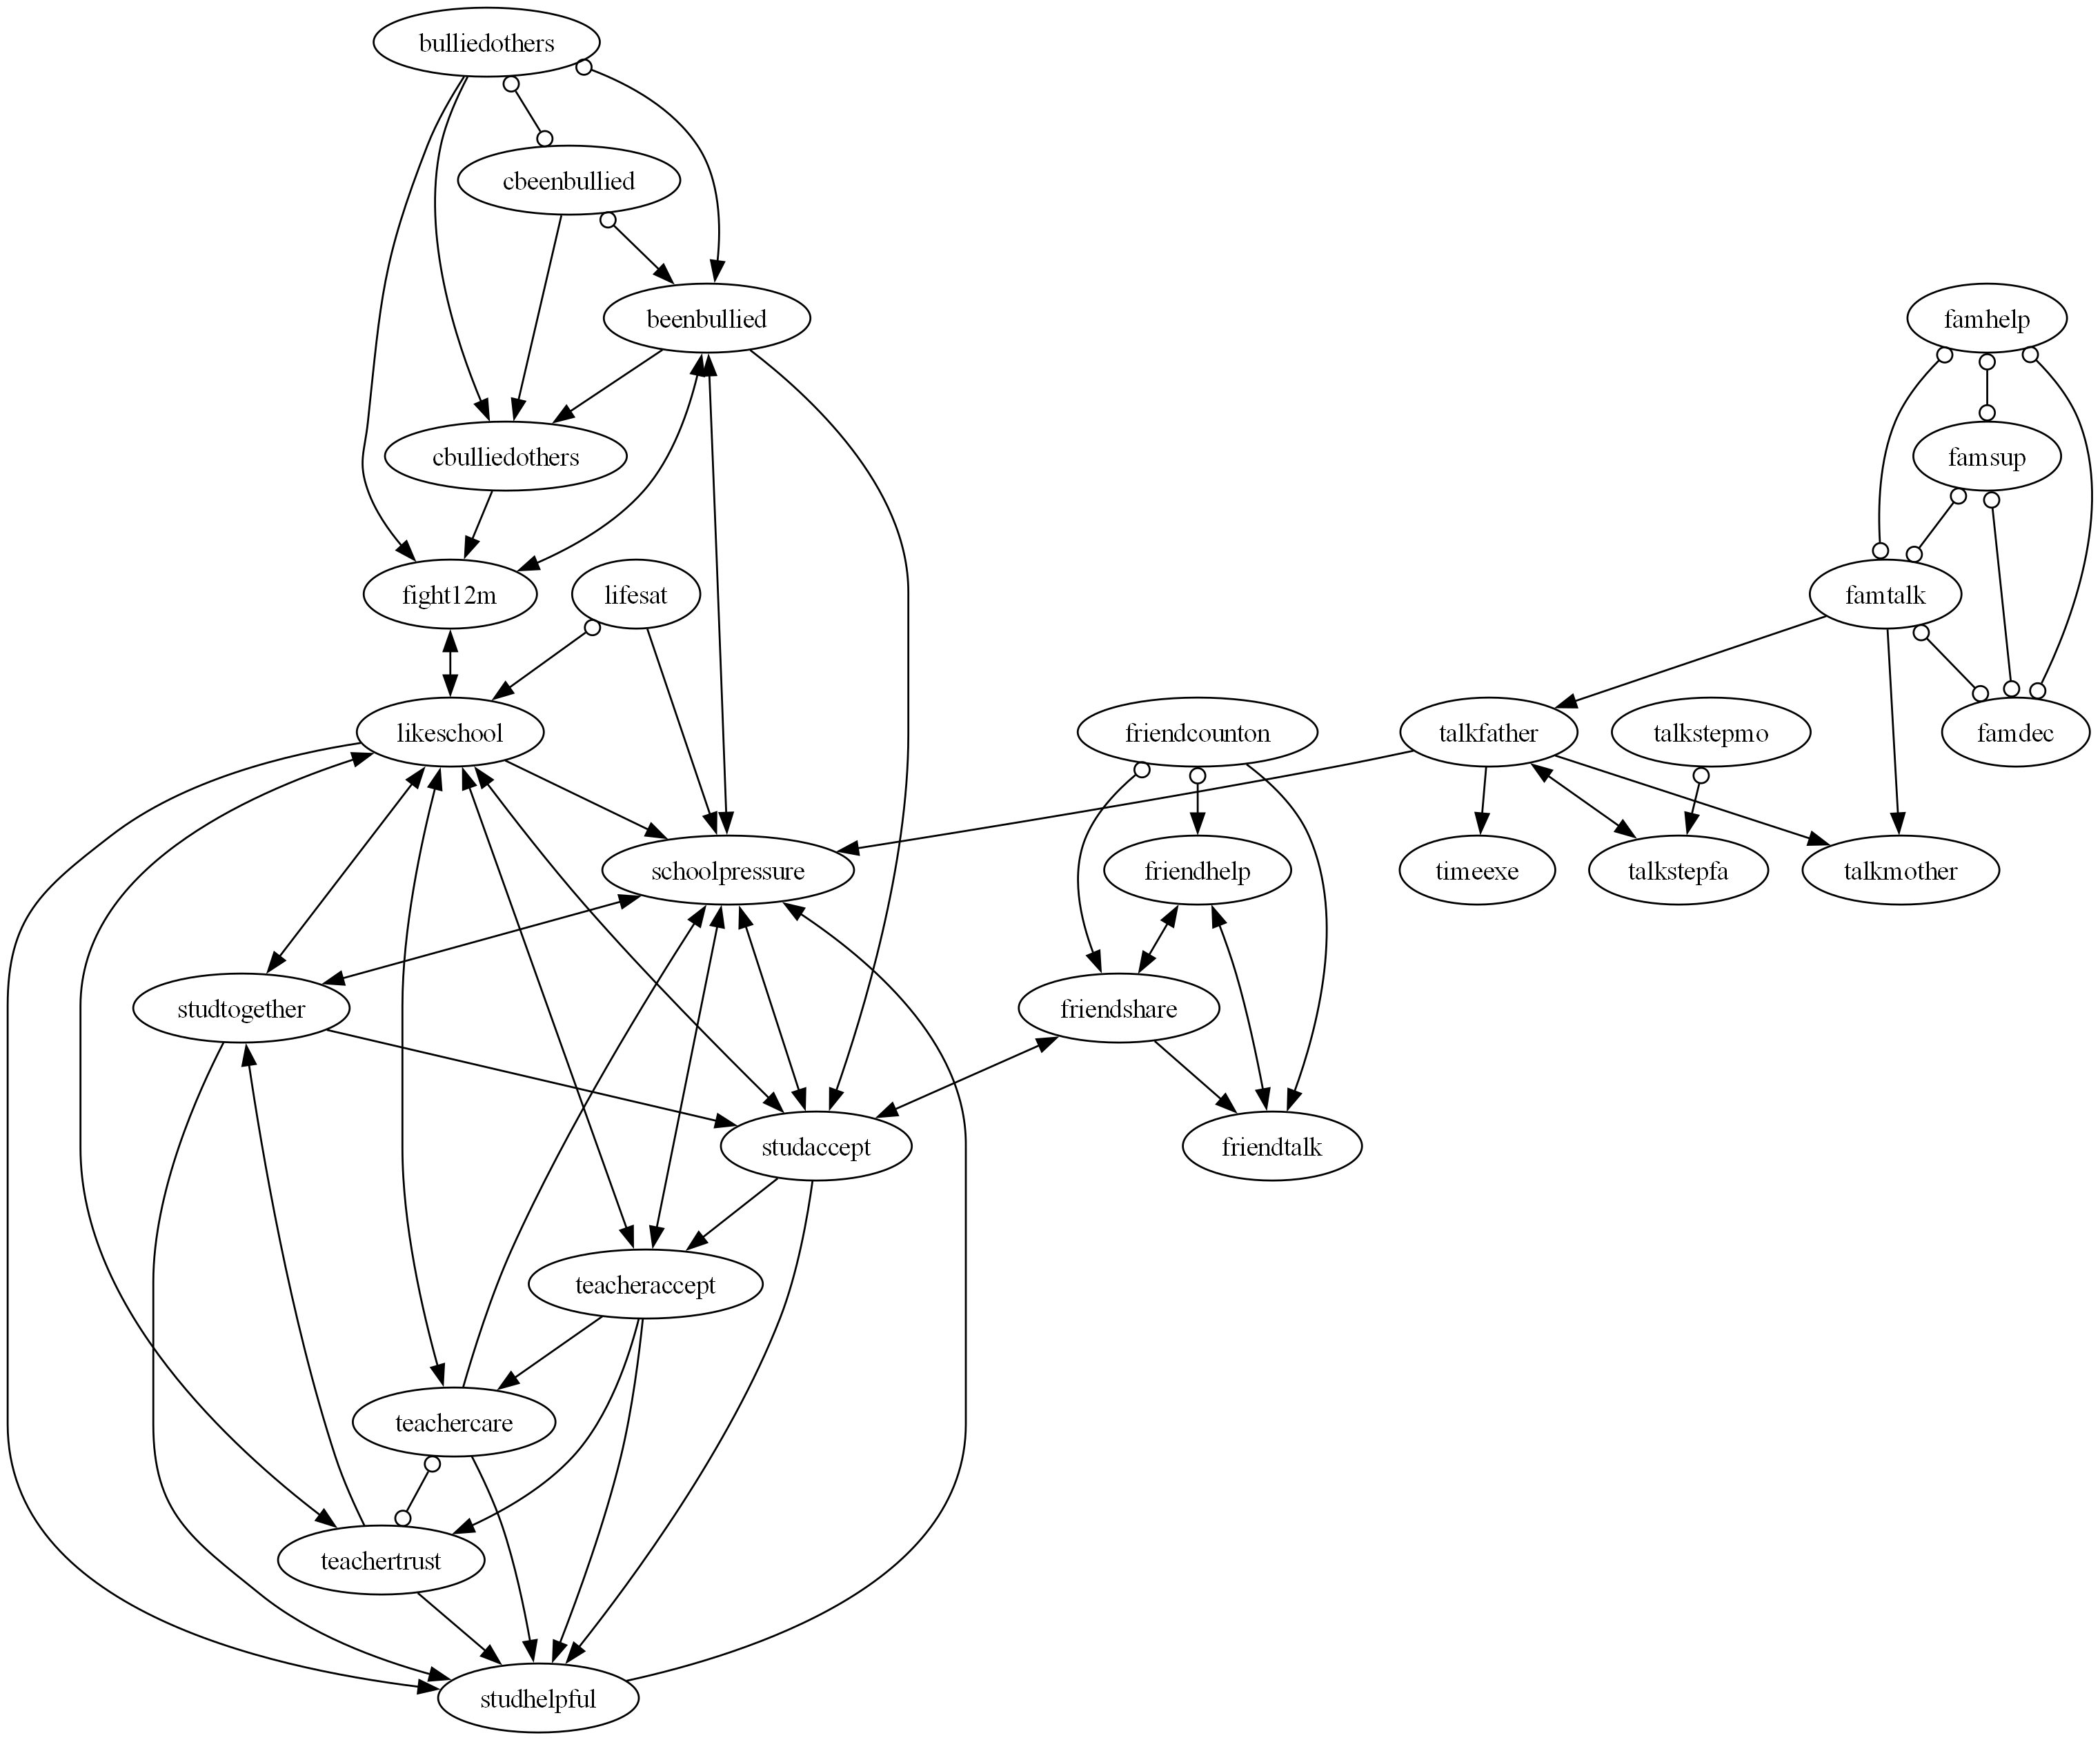
\includegraphics[width=0.8\textwidth]{Report/final_report/pictures/FCI_gsq_0.05_all_UA_27_talkmother.png}
    \caption{Findings from the FCI algorithm with $G^2$, performed at a significance level of 0.05.}
    \label{fig:fci_gsq_0.05all_UA_27_talkmother}
\end{figure}



\end{document}